% !TeX root = ../main.tex

\chapter{循环优化}

\section{循环优化简介}

循环是程序复杂度的主要来源,也是所有编程语言里必须支持的基本语句功能,对循环的优化通常是对程序性能影响最大的改进方式。

由于循环语句通常都是如下形式:
$$ \text{for} (i = \text{start}; i<\text{end};i = i+ step) $$

因此为了描述方便,本节术语约定如下:

1.用“迭代变量”代指循环中的变量$i$,

2.用“循环左边界”代指迭代变量的初值$i$,

3.用术语“循环右边界”代指迭代变量的结束判断条件,

4.用“迭代步长”代指每次循环中更新 $i$的变量step,

5.用 n 代指循环执行的次数${(end-start)}/{step} $。

编译原理中对于循环的常见优化有:

1. 循环不变量外提(loop-invariant code motion),把与循环迭代次数无关的计算语句移动到循环外。如循环体中的语句$invariant = constA * constB$

2. 循环展开(loop unrolling),把循环步长增大,把本来在循环中依次执行的若干条指令在一次循环中执行,这样可以提高并发性,减少分支预测的次数,从而在硬件级别提高程序的性能。

3. 删除归纳变量(inductive variable elimination),迭代变量及迭代变量的线性组合即归纳变量,对于复制语句j=t,如果在归纳变量j的所有引用点都可以用对t的引用代替对j的引用,在循环的出口处不活跃,则可以删除复制语句j=t,这可以通过复写传播优化实现。

下面着重介绍SSA形式下本项目的循环不变量外提算法。

\subsection{循环查找}

要实现上述的循环优化算法,第一步应是识别控制流程图中的循环结构。控制流程图中的循环具有以下特征,一,有唯一的入口节点,记为header,二,至少有一条回边,即从某个header支配的节点 n 通向 header 的路径,这两个条件是控制流程图中有循环的充要条件。

定义,假定CFG中存在一条回边n \Leftarrow header,循环由n, header 和其他所有不需要经过header就能到达n的节点组成。

事实上,控制流程图中的一个强连通分量就是一个循环。Tarjen算法\cite{doi:10.1137/0201010}是基于深度优先查找,对有向图的所有强连通分量顶点集的划分算法,可以使用该经典图论算法来进行循环查找,算法的伪代码描述如~\ref{algo:tarjen}。

\begin{algorithm}[htb]
  \small
  \SetAlgoLined
  \KwData{graph $G=(V,E)$}
  \KwResult{set of strongly connected components (sets of vertices)}
  
  index = 0\;
  stack = emptry\;
  \For{v in nodes}{
    \If{v.index is undefined}{
        strongconnect(v)\;
    }
  }
  \caption{访问模块生成IR}
  \label{algo:tarjen}
\end{algorithm}

Tarjen算法的核心在strongconnect函数,该函数的算法流程是,接受图中某一节点为参数,初始化该店的index为当前的时间戳,由于此时还未发现该节点的后代节点,初始化该节点在图中能达到的最早时间戳lowlink为其自己的时间戳。

从该点开始进行深度优先搜索,使用相同的时间戳发现和标记后代节点的序号index。将后代节点按照被访问的顺序入栈,在深度优先搜索的回溯过程返回至一个父节点时,由于已经获得了子节点的可达性信息,可以由下而上的更新父节点的lowlink为父子节点分别lowlink的最小值。

如果该节点的lowlink小于其index,说明该节点在控制流程图中可达被更早发现的节点,该类节点是某条由自身指向祖先节点的回边的头节点,也即该节点应该是循环体内的节点。

在整个深度优先搜索过程结束后,判断参数节点$v$的lowlink和index值,如果二者相同,就说明该节点是某个强连通分量的根节点,也即该循环的header,则在它之前出堆栈且还不属于其他强连通分量的节点构成了该节点所在的强连通分量,将栈中循环体中的元素逐个弹出直至发现$v$。

注意到Tarjen算法会对所有经过某次深度优先搜索后未被发现的节点开始一次搜索,所以Tarjen算法结束时,一定可以得到整个图的全部强连通分量连接情况。

 
\begin{algorithm}[htb]
  \small
  \SetAlgoLined
   v.index = index //当前最小index
   
   v.lowlink = index //初始化为当前可达的自己的index
   
   index = index + 1
   
   S.push(v)
 
   \For{(v,w) in  E}{
        \eIf{w.index is undefined}{
            //后继未访问过,深度优先访问
            
            strongconnect(w)
            
             v.lowlink = min(v.lowlink, w.lowlink)
            
            //更新该节点可达的最小index值
        }{
        \If{w in S}{
            //w已在栈S中,则其也在当前的强连通分量中
            
            v.lowlink = min(v.lowlink, w.index)
            }
        }
   }
   //深度优先搜索结束
   
    \If{v.lowlink = v.index}{
     // 若v是根则出栈,并得到一个强连通分量
        
        start a new strongly connected component
       
       \While{not w==v}{
            w = S.pop()
            
           add w to current strongly connected component
       }
       output the current strongly connected component
    }
  \caption{Tajen算法的strongconnect函数伪代码}    
  \label{algo:strongconnect}
\end{algorithm}

以图~\ref{fig:dfs}为例,说明循环发现的过程,假定从入口节点entry开始深度优先遍历,事实上,由于Tarjen算法会检查图中所有未被发现的节点,所以从任何一个图中节点开始遍历的结果相同。

表~\ref{tab:dfs}记录了深度优先搜索的过程中发现各个节点的时间戳index和从该节点回溯时确定的该节点在图中可达的最小时间戳lowlink值。

\begin{figure}[htb]
  \centering
  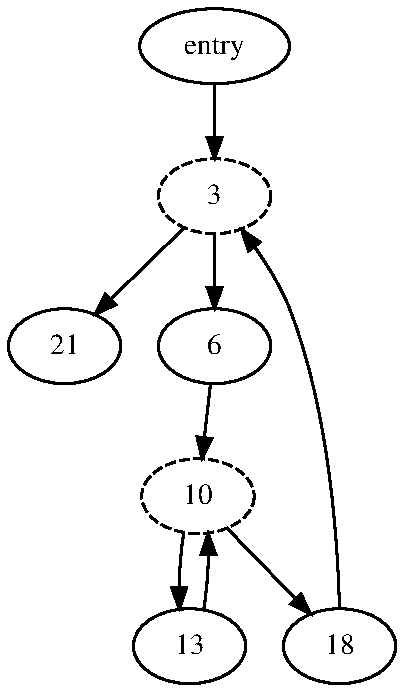
\includegraphics[width=0.5\textwidth]{figures/cfg.pdf}
  \caption{程序控制流程图}
  \label{fig:dfs}
\end{figure}

表中只描述了发现循环体\{10,13,18\}的过程:在节点10的回溯过程中,弹出在10之前入栈的节点13和18,由于10的index与lowlink相同,它们构成了一个循环。对于3号节点,同理。对于21号节点,虽然21号节点也会被当作一个强连通分量,但是其规模为1,无法构成循环。

\begin{table}[htb]
  \centering\small
  \caption{深度优先遍历发现内层循环的过程}
  \label{tab:dfs}
  \begin{tabular}{lcl}
    \toprule
    节点   & low link & index                           \\
    \midrule
    entry & 0 & 0   \\
    3 & 1 & 1       \\
    6 & 2 & 2       \\
    10 & 3 & 3      \\
    13 & 4 & 3      \\
    18 & 5 & 3      \\
    \bottomrule
  \end{tabular}
\end{table}


\section{循环不变量外提}

经过了循环查找,如果循环的某个节点中有条指令的所有源操作数为不变量,那么这条指令可以移动到循环外。具体而言,外提的不变量形式如下:

1. 把常量标记为不变量

2. 把只在循环外定值的变量标记为不变量

3. 把所有源操作数为上述两个条件定义的不变量的指令目的操作数定义为不变量

不变量外提算法是一个数据流分析的过程,按照上述次序标记循环中的不变量指令,迭代到不动点,最后的结果中,不变量指令和循环次数无关,因此可以移动到循环之外。

而外提的具体实现比较简单:只需要在循环的进入前新加一个基本块 LoopInvariant Area,把不变量指令提出到这个新的基本块中,然后调整该基本块的前驱后继关系,并把后续基本块中用到这个不变量指令的 $\phi$ 指令参数进行修改,重新使得 IR 合法。

该Pass类的run方法如下:

\begin{algorithm}[htb]
  \small
  \SetAlgoLined
  \KwResult{Mark and Move Loop Invariant}
  Changed = True
  
  Invariant= empty
  
  \While{Changed}{
    \For{all e in Instructions}{
        mark Const as Invariant\;
        mark Reached Value as Invariant\;
        \If{all of e.operations is Invariant}{
            mark e.value as Invariant\;
        }
    }
    \If{IR\_new equals to IR}{
        Changed = False\;
    }
  }
  do Loop Invariant Motion\;
  
  \caption{Loop Invariant Motion}
  \label{algo:loopinvar}
\end{algorithm}


值得注意的是,如果循环的条件不满足,但是我们进行了外提,那么对于源代码级的程序会产生多余的变量赋值,考虑循环内外都对某个变量进行了赋值,而循环又因为条件为假不会进入的情况,如果直接进行外提,编译器会错误的产生一个新赋值,这将使得循环后用到这个赋值的地方出错,那么,我们是不是应该把循环的条件部分也外提一次,即在基本块 LoopInvariant Area前设置一个 if 条件基本块呢?比如这个案例:

\begin{verbatim}
int n = 10;
int i = 1;
int step = 0;
while (i > n){  // FALSE condition, cannot execute!
	int step = 4*i; 
	// code
}
k = step;
// use of variable k
\end{verbatim}

如果我们外提时没有添加if,那么编译器会错误的产生一个新赋值 step = 4,这将使得下方的 k 出错!

\begin{verbatim}
int n = 10;
int i = 1;
int step = 0;
// if (i>n)
    int step = 4*i;
while (i > n){ 
	// code
}
k = step;   // ERROR HERE
// use of variable k

\end{verbatim}

事实上,这种情况是不会发生的,因为对于SSA形式,每个变量只有一次被赋值的机会,出现在循环内的赋值就意味着不会再出现对此变量的其他赋值语句,经过外提后只有用得上或者用不上两种情况,而不会产生上述的覆盖出错。

所以来自源代码级的外提导致的错误赋值的情况没有必要在SSA形式下进行考虑,验证一下,由上述代码生成控制流程图~\ref{fig:motion0}:

\begin{figure}[htb]
  \centering
  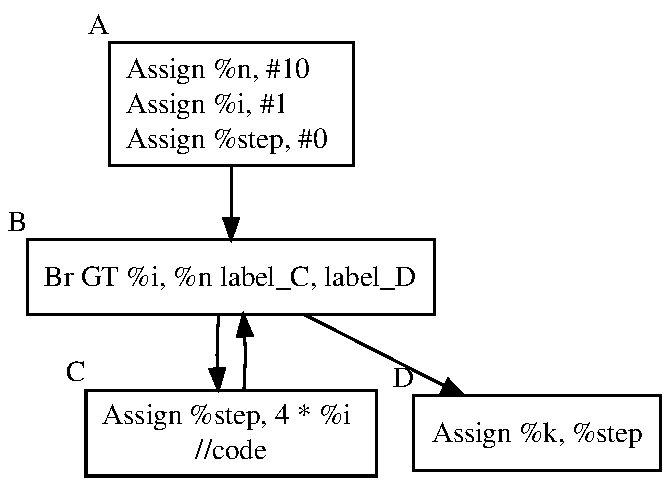
\includegraphics[width=0.8\textwidth]{figures/codeMotion.pdf}
  \caption{直接从源代码得到的控制流程图}
  \label{fig:motion0}
\end{figure}

注意,现在是SSA的形式,我们需要满足SSA的要求,即每个变量只能被赋值一次。检查整个控制流程图,可以看到虚拟变量\%step在基本块A和C中被赋值了两次,这违反了SSA的定义,所以这并不是合法的SSA控制流程图。

为了符合单赋值的要求,把基本块C中的虚拟变量\%step重命名为\%step\_new,在有多个对step进行定值的基本块B中插入一条关于step的$\phi$指令,并将基本块D中对\%step的使用修改为\%step\_phi,得到图~\ref{fig:motion1}。

\begin{figure}[htb]
  \centering
  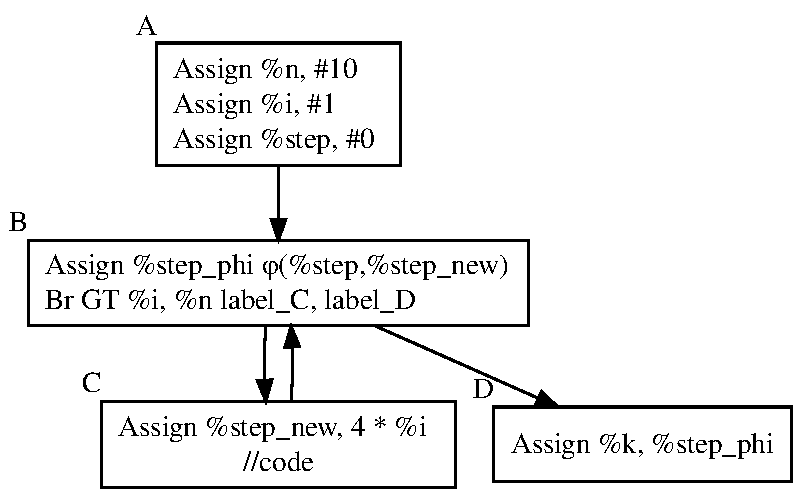
\includegraphics[width=0.9\textwidth]{figures/codeMotion_phi.pdf}
  \caption{符合静态单赋值要求的控制流程图}
  \label{fig:motion1}
\end{figure}

这样一来就是正确的SSA形式,进行代码外提之后,得到图~\ref{fig:motion2}。

\begin{figure}[htb]
  \centering
  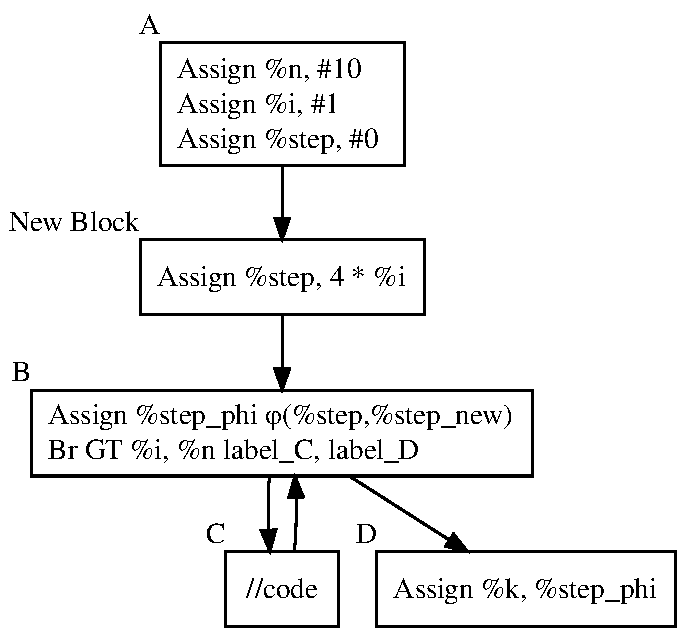
\includegraphics[width=0.8\textwidth]{figures/post_codeMotion.pdf}
  \caption{进行代码外提后的控制流程图}
  \label{fig:motion2}
\end{figure}

可以发现基本块D中step的值实际上取决于虚拟变量\%step\_phi,也即实际的运行时控制流决定了step的值。所以说SSA形式上变量外提时,是不需要添加if条件的。


\section{循环多线程化}

\subsection{简介}

本项目对于最简单的并行计算情况,利用了树莓派ARM EABI 架构的4核处理器,开发了创新多线程框架,与经典框架 OpenMP 对比,其优点有:

1.共享栈空间:不需要将被并行化的区域拆分出来变成函数

2.框架更加易于实现:不需要保存上下文和维护各种信息

3.更便于代码变换:只需在 IR 前后就地插入 Call MTStart和 MTStart End

4.更高的运行性能:栈上的资源仍然可以直接通过栈指针加偏移访问

本项目的多线程框架类似于GPU的设计思想,仅针对不需要线程通信的情况,即每个线程之间互相不会产生干扰,彼此读写属于自己的区域,这也是上文所述线程之间可以共享栈中的局部变量,而不需要互斥锁等同步机制的原因。

举例来说,对规模为100的数组A的每个元素进行平方运算,由于这个问题可以划分为4个独立进行互不干扰的子问题,编译器可以通过系统调用创建4个线程并行独立地共同完成这个问题:一号线程读写前25个元素,二号线程读写26到50个元素,以此类推,从而充分利用树莓派的4核处理器,进一步提高机器码性能。

\subsection{多线程框架代码实现}

下面介绍如何在ARM EABI Linux的系统上通过汇编码创建共享栈空间的子线程。

首先,多线程必然需要系统调用的支持,Linux在arm/EABI的system call约定是R7作为系统调用号寄存器,使用寄存器R1到R6传递参数,R0作为返回值。其次,要注意区分Windows系统和Linux对线程的不同设计,Linux系统的线程设计可以表述为,线程只不过是共享虚拟地址空间和文件描述符表的进程,定义上线程之间共享除寄存器、栈之外的所有资源。操作系统和底层硬件天然地保证了线程不会共享寄存器,TLS不是必须的,本项目又使得线程之间共享栈空间,更关键的是,由于共享栈空间,使得栈指针寄存器共享,所以局部变量也被共享,切换的开销大大缩小。

clone跟fork都是创建子进程(线程),区别在于clone能更详细的定制子进程和父进程共享的内容:如虚拟内存地址空间,文件描述符表,因而本项目使用clone系统调用,设置参数clone\_flags为父子线程共享栈空间,不必共享其他资源。

clone对父进程返回所创建的子进程的pid,如果失败,返回-1,这正是程序区分父子线程的关键。

\begin{verbatim}
    sub r2, r2, \#1     
    cmp r2, \#0         
    beq .finish			
    mov r7, \#120	    
    mov r0, \#273	    
    mov r1, sp	        
    swi \#0         ; system call
    cmp r0, \#0		    
    bne .mtstart
\end{verbatim}

说明:

前三条指令表示利用r2统计已经创建的线程数:r2事先初始化为4,每循环一次减一,当r2等于0时,创建子线程完毕,

第四条指令为设置系统调用参数号为120,即clone的系统调用号。

第五条指令表示设置系统调用的首个参数clone\_flags,273的十六进制即0x0111,在Linux系统代码中表示共享虚拟存储的子进程,显然由于SysY中无无文件读写等功能,所以只需共享最基本的虚存空间即可。
    
第六条指令中,由于系统调用clone的参数r1为子线程栈地址,通常框架下子线程拥有自己独立的栈空间来存储自己的局部变量,并且防止误写父线程的局部变量,但是该项目的多线程框架下无需担心此问题,所以只需要把子线程的栈指针设置为父线程的栈指针sp即可。

第七条swi \#0是arm EABI的软中断指令,类似x86的int 0x80。从这条指令之后,父子线程会开始并行执行,为了区分父子线程,利用上文提到的clone对父子线程返回的值r0不同:对子线程返回0,子线程会顺序执行,离开子线程创建的汇编代码区域;对父线程返回子线程pid,Linux下的创建成功pid是一个非负整数,因而必然会导致父线程回到第一条指令,对r2减一,判断所有子线程是否已经创建完毕。